%!TEX root = TQFTnotes.tex
%%%%%%%%%%%%%%
\chapter{2d TQFT with defects}\label{c:2d-defects}
References: \cite{cdr}: review article; 
\cite{dkr} one of first constructions;
\cite{carqueville}

FIXME

So far we only considered TQFTs defined on (unstratified) manifolds. Even the manifolds with corners, that we used to motivate the definition of extended TQFT, were meant to be glued back to form an unstratified manifold. Such (extended) TQFTs can be considered as describing physics on a homogenous spacetime. It is then natural to consider more general physical systems, where the different parts of the spacetime are described by different TQFTs. The codimension 1 surface separating the homogenous parts can be thought of as a defect that makes the spacetime non-homogenous. This motivates us to define the notion of TQFT with defects.

\begin{figure}[ht]
	\centering
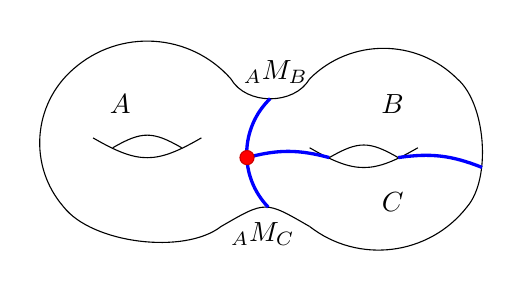
\begin{tikzpicture}[scale=0.5]
	
	\pgfdeclarelayer{nodelayer}
	\pgfdeclarelayer{edgelayer}
	\pgfdeclarelayer{labels}
	\pgfsetlayers{edgelayer,nodelayer,labels,main}
	\tikzset{
		none/.style={},
		defect/.style={draw=blue, line width=1.2pt},
		junction/.style={circle, fill=red, draw=red!80!black, line width=0.4pt, inner sep=1.8pt},
	}
	
	\begin{pgfonlayer}{nodelayer}
		\node [style=none] (4) at (1, 0) {};
		\node [style=none] (5) at (3.75, 0) {};
		\node [style=none] (B) at (1.5, -0.25) {};
		\node [style=none] (C) at (3.25, -0.25) {};
		\node [style=none] (8) at (-1.25, -2) {};
		\node [style=none] (R) at (1, -2) {};
		\node [style=none] (10) at (-5.25, -1.5) {};
		\node [style=none] (11) at (-5, 2) {};
		\node [style=none] (P) at (-1, 1.75) {};
		\node [style=none] (Q) at (1, 1.75) {};
		\node [style=none] (14) at (4.75, 1.75) {};
		\node [style=none] (15) at (5, -1.5) {};
		\node [style=none] (16) at (-4.5, 0.25) {};
		\node [style=none] (17) at (-1.75, 0.25) {};
		\node [style=none] (18) at (-4, 0) {};
		\node [style=none] (19) at (-2.25, 0) {};
		\node [style=none] (E) at (0, 1.25) {};
		\node [style=none] (F) at (-0.05, -1.51) {};
		\node [style=junction] (A) at (-0.59, -0.25) {};
		\node [style=none] (D) at (5.38, -0.5) {};
	\end{pgfonlayer}
	\begin{pgfonlayer}{edgelayer}
		\draw [bend right, looseness=1.25] (4.center) to (5.center);
		\draw [bend left, looseness=1.25] (B.center) to (C.center);
		\draw [bend left=45] (11.center) to (P.center);
		\draw [bend right=60] (P.center) to (Q.center);
		\draw [bend left=45] (Q.center) to (14.center);
		\draw [bend left=45, looseness=0.75] (14.center) to (15.center);
		\draw [bend left=45] (15.center) to (R.center);
		\draw [bend right, looseness=1.50] (R.center) to (8.center);
		\draw [bend right=315, looseness=0.75] (8.center) to (10.center);
		\draw [bend left=45] (10.center) to (11.center);
		\draw [bend right, looseness=1.25] (16.center) to (17.center);
		\draw [bend left, looseness=1.25] (18.center) to (19.center);
		\draw [defect,bend right=45] (E.center) to (F.center);
		\draw [defect,bend left=15] (A.center) to (B.center);
		\draw [defect,bend left=15] (C.center) to (D.center);
	\end{pgfonlayer}
	\begin{pgfonlayer}{labels}
		\node[above, xshift=2pt, yshift=2pt] at (E) {$ _AM_B$};
		\node[below, xshift=-2pt, yshift=-2pt ] at (F) {$ _AM_C$};
		\node[below, xshift=-40pt, yshift=-2pt ] at (P) {$A$};
		\node[below, xshift=30pt, yshift=-2pt ] at (Q) {$B$};
		\node[above, xshift=30pt, yshift=2pt ] at (R) {$C$};
	\end{pgfonlayer}
\end{tikzpicture}
  \caption{A stratified manfold decorated with algebras $A$,$B$ and $C$ on different regions.}
\label{f:stratified_pretzel}
\end{figure}

\begin{enumerate}
	\item Manfold $M$ with a stratification
	
	$M=M^0 \cup M^1 \cup M^2$
	
	Here $M^0$ are the 2 dimensional open sets whose boundary constitutes $M^1$.  Stratum $M^1$ is codimension 1 subspace with boundary $M^2$. Similarly, $M^2$ are codimension 2 subspace at the boundary of $M^1$. ( For higher dimensional manifolds, the stratification can have higher codimension strata.)
	
	For example, in the Figure \ref{f:stratified_pretzel}, the stratum $M^0$ consists of three regions, labelled as $A$,$B$, and $C$. The stratum $M^1$ consists of blue lines. The red dot at the intersection of blue lines belongs to the stratum $M^2$.
	
	\item Coloring
	\begin{itemize}
		\item Connected components of $M^0$ are colored by semisimple symmetric Frobenius algebras. In Figure \ref{f:stratified_pretzel}, $A$, $B$, and $C$, are three such algebras.
		\item Connected components of $M^1$ are colored by bimodules. These 1-dimensional components ( called defects ) come with a orientation. If the regions to the left and to the right of a defect are colored by algebras $A$ and $B$ respectively, the defect is labelled by a bimodule $ _AM_B$. If we change the orientation of defect, it is labelled by $ _BM^{*}_A$ bimodule. $M^*$ is dual to $M$, as expected from orientation reversal.
		\item The vertices ( also called junctions ) are points where two or more defects meet. For each vertex $u \in D^2$, we need a multilinear map $\varphi_u: M^1 \otimes_{A_2}  M^2 \otimes_{A_3} M^3 \otimes_{A_4} M^4 \rightarrow  \kk$.
	\end{itemize}
\end{enumerate}

\clearpage